
\chapter{Introducción al scraping en la web: Marco teórico}
\label{cha:introduccion al scraping en la web} 

\section{¿Que es realmente el web scraping?}
\label{sec:Que es realmente el web scraping}


La web es la estructura de datos mas grande en la actualidad, una gran cantidad de datos es almacenada en 
algun lugar esperando a ser consultada. Tradicionalmente la extracción de dicha información se ha 
realizado a traves del copy-paste, aunque en ocasiones pueda ser la unica manera, esta es una tecnica muy
poco productiva e ineficiente de obtener información. Hasta ahora, no ha existido un termino oficial de la 
palabra, pero podemos definir \textit{web scraping} o como \emph{"técnica utilizada mediante 
programas de software para extraer información de sitios web."} \cite{web-scraping-wikipedia}

[En esencia, el web scraping se utiliza para obtener datos no estructurados de páginas web y
transfórmelo en una presentación estructurada o para almacenarlo en una base de datos externa.
También se considera una técnica eficiente para recopilar macrodatos, donde la recopilación de grandes cantidades de datos es importante.]

\begin{figure}[tphb]
  		   \centering
     		   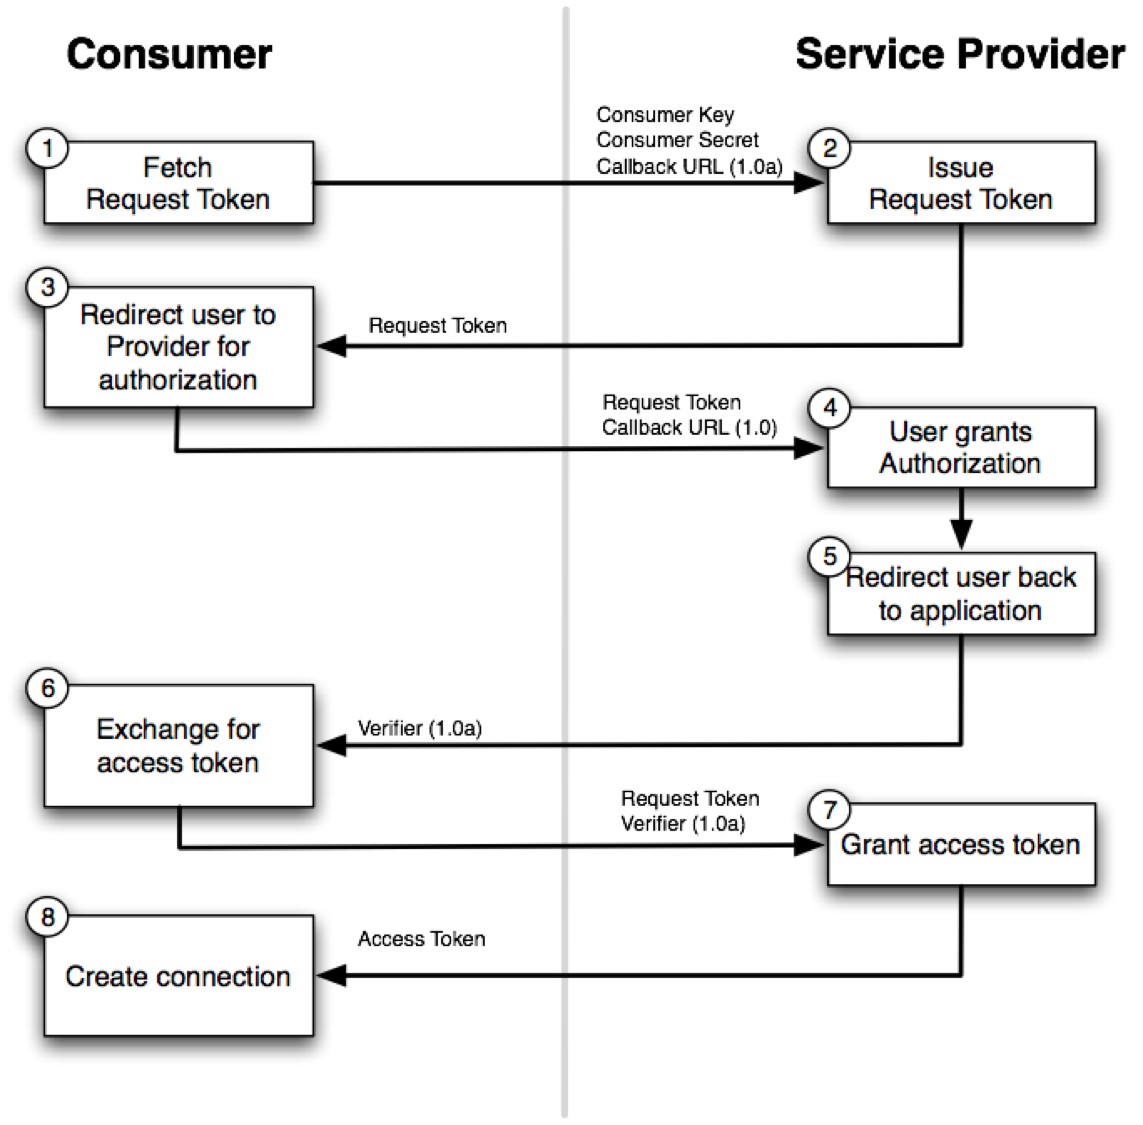
\includegraphics[width=4.5in]{Oauth1a.png}
  		   \caption{Funcionamiento de Oauth1a}
  		   \label{img:oauth1a}
\end{figure}






